% Volume III: Probability, Statistics, Information, and Causality
% Continuity note for Chapter 18.
% Previous dependencies: Chapter 13's probability spaces, random variables, joint/conditional distributions, and covariance; Chapter 14's discrete, continuous, Gaussian, and exponential-family models; Chapter 15's expectation, conditioning, Bayes updates, and decision rules; Chapter 16's concentration and high-dimensional probability intuition; Chapter 17's likelihood, log-likelihood, predictive risk, and Fisher information as likelihood curvature.
% New durable concepts: surprise, entropy, log base and information units, maximum entropy on a finite support, continuous entropy caveat, cross-entropy, KL divergence, Gibbs inequality, support mismatch, mutual information, conditional entropy, data processing for Markov chains, statistical manifold, Fisher metric, local KL curvature, and natural gradient.
% Forward hooks: Neural coding reuses entropy and mutual information to quantify stimulus-response information; variational inference reuses KL divergence and cross-entropy as optimization objectives; representation learning reuses information bottlenecks and contrastive objectives; experimental design reuses Fisher information to choose measurements that distinguish nearby hypotheses.
% Notation commitments: Discrete distributions are written p(x), q(x) on a finite or countable support \mathcal X unless stated otherwise; logs use base 2 and information is measured in bits in Sections 18.1--18.3 unless natural logs are explicitly named; the convention 0\log 0=0 is used; entropy is H(X) or H(p); cross-entropy is H(p,q); KL divergence is D_{\mathrm{KL}}(p\|q); mutual information is I(X;Y); Fisher information is \mathcal I(\theta) to avoid collision with mutual information.
% Figure plan: four ImageGen raster figures under imagegen-figures/ch18-* are referenced: entropy as average surprise for 18.1; KL/cross-entropy mismatch for 18.2; mutual information as joint-vs-product structure for 18.3; Fisher geometry on a Bernoulli statistical manifold for 18.4.
\section{Chapter 18: Information Theory and Information Geometry}
\label{ch:information-theory-information-geometry}

Chapters 13--17 turned uncertainty into a mathematical object. We defined random variables and distributions, learned how expectations and conditioning summarize information, used limit theorems to control sampling variability, and used likelihood to fit statistical models. Chapter 18 asks a different but closely related question: how much uncertainty is present, how different are two distributions, and how much information does one variable carry about another?

The answer is not one number for every situation. Entropy measures uncertainty in a distribution. KL divergence measures the directed mismatch between a true distribution and an approximation. Cross-entropy is the expected coding or prediction loss when the approximation is used. Mutual information measures dependence between variables. Fisher geometry describes the local shape of a family of probability distributions.

\paragraph{Chapter problem.}
How can we measure uncertainty, distinguishability, coding cost, dependence, and local geometry in probability models in a way that supports neuroscience, machine learning, and statistical decision making?

\paragraph{Section map.}
Section 18.1 begins with surprise and entropy. Section 18.2 defines KL divergence and cross-entropy as distribution mismatch and expected code length. Section 18.3 defines mutual information as the KL divergence between a joint distribution and the independent product of its marginals. Section 18.4 turns a parameterized family of distributions into a statistical manifold whose local metric is Fisher information.

\subsection{18.1 Entropy and uncertainty}

\paragraph{Motivating question.}
How much uncertainty does a random variable contain before we observe its value, and how many bits should we expect to need to encode the outcome?

\paragraph{Beginner setup.}
The basic unit is \emph{surprise}. If an outcome has probability \(p(x)\), its surprise is
\[
 -\log p(x).
\]
Rare outcomes are more surprising than common outcomes. If the logarithm uses base \(2\), surprise is measured in bits. An event with probability \(1/2\) carries \(1\) bit of surprise; an event with probability \(1/8\) carries \(3\) bits.

Entropy is average surprise. It solves the problem of summarizing the uncertainty of an entire distribution rather than one realized outcome. A fair coin has more entropy than a coin that lands heads with probability \(0.9\), because before flipping the fair coin we are less able to predict the result.

What to keep in mind: entropy is a property of a distribution, not of a single sample. After an outcome happens, the surprise of that outcome is known, but the entropy still describes the uncertainty that was present before observation.

\begin{figure}[htbp]
\centering
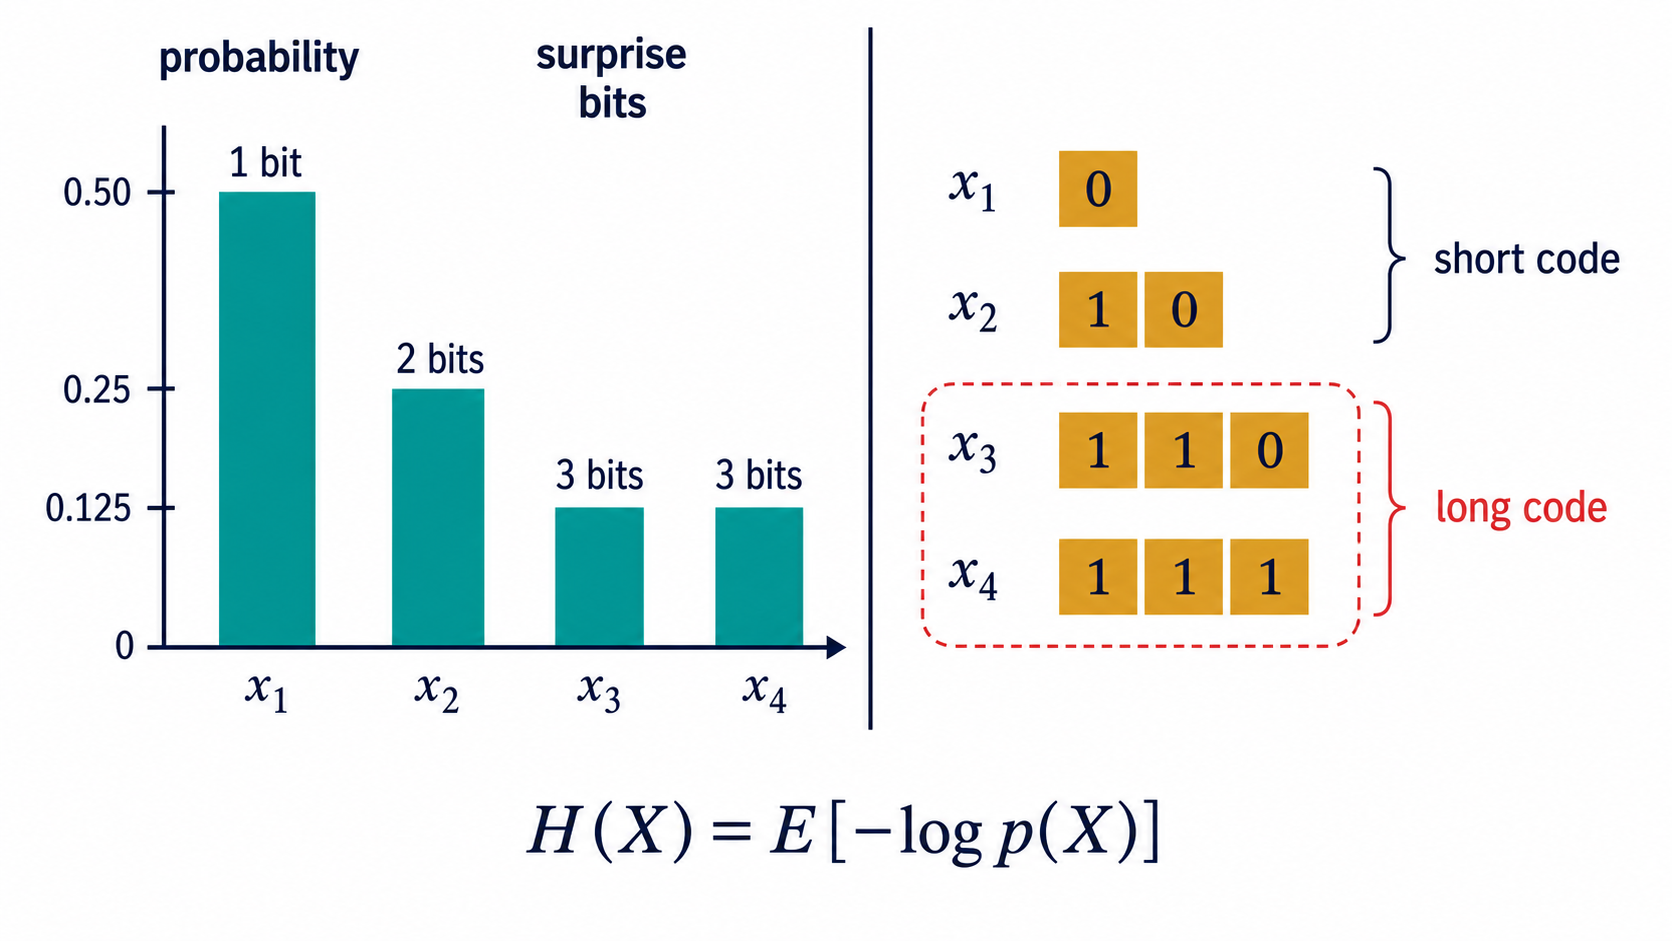
\includegraphics[width=0.98\linewidth]{imagegen-figures/ch18-entropy-average-surprise.png}
\caption{Entropy is average surprise. Common outcomes have small surprise and can be assigned short codes; rare outcomes have larger surprise and need longer codes. The expected code length is the probability-weighted average of the surprise values.}
\label{fig:ch18-entropy-average-surprise}
\end{figure}

\paragraph{Formal setup.}
Let \(X\) be a discrete random variable with finite or countable support \(\mathcal X\), and let
\[
p(x)=P(X=x),\qquad x\in\mathcal X.
\]
For a logarithm with base \(b>1\), the entropy of \(X\) is
\[
\boxed{
H_b(X)=H_b(p)
=-\sum_{x\in\mathcal X} p(x)\log_b p(x)
=\mathbb E[-\log_b p(X)].
}
\]
When \(b=2\), entropy is measured in bits. When \(b=e\), entropy is measured in nats. This chapter usually uses base \(2\) in Sections 18.1--18.3.

The support convention is
\[
0\log 0=0,
\]
which means that impossible outcomes contribute no average surprise. This convention follows from the limit \(p\log p\to 0\) as \(p\downarrow 0\).

For a continuous random variable with density \(p(x)\), one can define differential entropy
\[
h(X)=-\int p(x)\log p(x)\,dx,
\]
but it is not the same kind of object as discrete entropy. Differential entropy depends on units and coordinate transformations, and it can be negative. For that reason, this beginner section treats discrete entropy as the primary object and uses continuous entropy only with caution.

\paragraph{Core intuition.}
Figure~\ref{fig:ch18-entropy-average-surprise} shows two equivalent pictures. On the left, probabilities determine surprise values. On the right, the same logic appears as coding: common outcomes deserve short codewords, rare outcomes can tolerate longer codewords because they occur less often. Entropy is the expected code length of an ideal code, up to the integer-length details of real coding schemes.

A common misconception is that entropy is the same as variance. Variance measures spread around a numerical mean, so it requires numerical values and units. Entropy only needs probabilities. The outcomes could be class labels, words, spike-count bins, or latent states. Another misconception is that high entropy means "disorder" in a vague sense. In this course, high entropy means high average surprise under a specified probability model.

This section uses Chapter 13's random variables and Chapter 15's expectation. It prepares cross-entropy and KL divergence in Section 18.2, mutual information in Section 18.3, and coding interpretations in neural and machine-learning models.

\paragraph{Main theorem: maximum entropy on a finite support.}
Suppose \(X\) has \(m\) possible outcomes and no other constraints are imposed. Then
\[
\boxed{
H(X)\le \log_2 m,
}
\]
with equality exactly when \(p(x)=1/m\) for every outcome.

\emph{Proof sketch.}
Write the probabilities as \(p_1,\ldots,p_m\), with \(p_i\ge 0\) and \(\sum_i p_i=1\). To find an interior maximum of
\[
H(p)=-\sum_{i=1}^m p_i\log_2 p_i
\]
under the constraint \(\sum_i p_i=1\), use a Lagrange multiplier:
\[
\mathcal L(p,\lambda)
=-\sum_{i=1}^m p_i\log_2 p_i+\lambda\left(\sum_{i=1}^m p_i-1\right).
\]
For \(p_i>0\),
\[
\frac{\partial \mathcal L}{\partial p_i}
=-\left(\log_2 p_i+\frac{1}{\ln 2}\right)+\lambda.
\]
Setting all partial derivatives to zero implies that all \(\log_2 p_i\) are equal, so all \(p_i\) are equal. The constraint then gives \(p_i=1/m\). Since entropy is concave as a function of \(p\), this stationary point is the global maximum. Its value is
\[
H(p)=-m\left(\frac{1}{m}\right)\log_2\left(\frac{1}{m}\right)
=\log_2 m.
\]
The mechanism is that, without any additional information, spreading probability uniformly maximizes average surprise.

\paragraph{Worked examples.}
\emph{Small numerical example.}
A fair coin has distribution \(p(H)=p(T)=1/2\). Its entropy is
\[
H(X)=-2\left(\frac12\log_2\frac12\right)=1\ \text{bit}.
\]
A biased coin with \(p(H)=0.9\) and \(p(T)=0.1\) has entropy
\[
H(X)=-0.9\log_2(0.9)-0.1\log_2(0.1)\approx 0.469\ \text{bits}.
\]
The biased coin is not uncertainty-free, but it is much easier to predict.

\emph{Coding example.}
For the four-outcome distribution in Figure~\ref{fig:ch18-entropy-average-surprise},
\[
p=(0.5,0.25,0.125,0.125).
\]
The surprise values are \(1,2,3,3\) bits, so
\[
H(p)=0.5(1)+0.25(2)+0.125(3)+0.125(3)=1.75\ \text{bits}.
\]
This is the ideal average code length suggested by the distribution.

\emph{Machine-learning example.}
A classifier that outputs \(p_\theta(y\mid x)=(0.98,0.01,0.01)\) over three classes is confident and has low predictive entropy. A classifier that outputs \((1/3,1/3,1/3)\) has entropy \(\log_2 3\) bits and is maximally uncertain among three classes. Entropy therefore becomes a diagnostic for uncertainty, calibration, and active learning.

\emph{Neuroscience example.}
Let \(R\) be a binned spike count for one neuron in a fixed time window. If the response distribution \(p(r\mid s)\) under stimulus \(s\) is concentrated on one count, then \(H(R\mid S=s)\) is low. If many response counts are plausible, the conditional response entropy is high. The random variable is neural response \(R\), the distribution is the trial-to-trial response distribution, and entropy summarizes response variability.

\paragraph{ML/DL/neuroscience connections.}
In supervised learning, entropy of a predicted label distribution measures how uncertain the model is about its output. In language modeling, entropy rate measures average uncertainty per token under a text distribution. In neuroscience, response entropy measures variability in neural activity, while stimulus entropy measures the uncertainty in the experimental input ensemble. These are not just metaphors: the mathematical object \(p(x)\) becomes a label distribution, a token distribution, a spike-count distribution, or a stimulus distribution, and \(H(p)\) is the same probability-weighted average surprise in each case.

\paragraph{Exercises.}
\begin{enumerate}[label=\textbf{18.1.\arabic*.}, leftmargin=*]
\item \textbf{Mechanical.} Compute the entropy in bits of a random variable with probabilities \((1/2,1/4,1/4)\).
\item \textbf{Proof or derivation.} Use the Lagrange-multiplier argument in this section to show that the maximum entropy distribution on three unconstrained outcomes is uniform.
\item \textbf{Numerical/computational.} Write down the entropy values for Bernoulli\((\theta)\) at \(\theta=0.1,0.5,0.9\). Explain why the first and third values match.
\item \textbf{Interpretation.} A neural response distribution has entropy near zero for one stimulus and high entropy for another. What does that say about trial-to-trial response variability under each stimulus?
\item \textbf{Debug the misconception.} A student says, "The outcome \(x_3\) has entropy \(3\) bits." Correct the statement using the distinction between surprise and entropy.
\end{enumerate}

\subsection{18.2 KL divergence and cross-entropy}

\paragraph{Motivating question.}
If data are generated by one distribution \(p\) but we predict or encode them using another distribution \(q\), how much extra cost does the mismatch create?

\paragraph{Beginner setup.}
Entropy assumes the code or predictor is matched to the true distribution. In practice, we usually use an approximation. A classifier uses predicted probabilities \(q_\theta(y\mid x)\), not the unknown true conditional distribution. A variational inference method uses an approximate posterior \(q(z)\), not the exact posterior. A neural encoding model uses a fitted response distribution \(q(r\mid s)\), not the true response law.

Cross-entropy measures the expected code length when outcomes from \(p\) are encoded as if \(q\) were correct:
\[
H(p,q)=-\sum_x p(x)\log q(x).
\]
KL divergence measures the extra cost beyond the best possible code for \(p\):
\[
D_{\mathrm{KL}}(p\|q)=H(p,q)-H(p).
\]

What to keep in mind: KL divergence is directed. Usually \(D_{\mathrm{KL}}(p\|q)\neq D_{\mathrm{KL}}(q\|p)\). It is a mismatch measure, not an ordinary distance.

\begin{figure}[htbp]
\centering
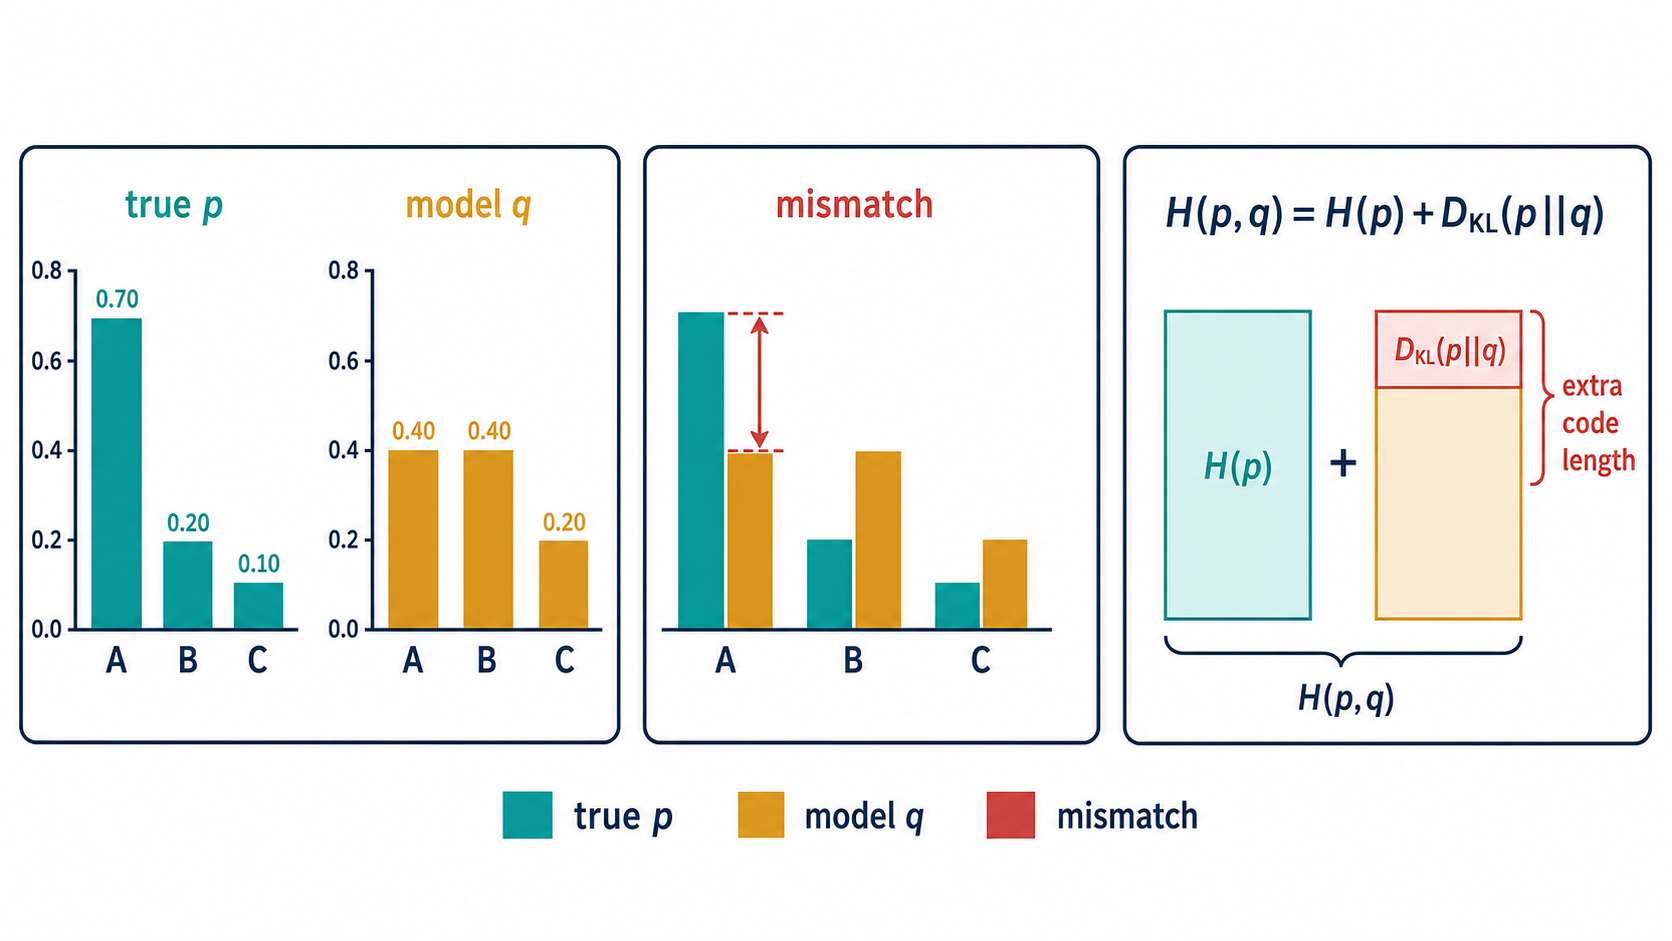
\includegraphics[width=0.98\linewidth]{imagegen-figures/ch18-kl-cross-entropy.png}
\caption{Cross-entropy is the expected code length when a model distribution \(q\) is used for data distributed as \(p\). KL divergence is the extra code length caused by mismatch. When \(q\) assigns too little probability to outcomes that occur often under \(p\), the penalty is large.}
\label{fig:ch18-kl-cross-entropy}
\end{figure}

\paragraph{Formal setup.}
Let \(p\) and \(q\) be discrete distributions on the same support \(\mathcal X\). Assume
\[
p(x)>0\quad\Longrightarrow\quad q(x)>0.
\]
If this condition fails, then \(q\) assigns zero probability to an event that can occur under \(p\), and the KL divergence \(D_{\mathrm{KL}}(p\|q)\) is infinite.

The cross-entropy from \(p\) to \(q\) is
\[
\boxed{
H(p,q)=-\sum_{x\in\mathcal X}p(x)\log_2 q(x).
}
\]
The KL divergence from \(p\) to \(q\) is
\[
\boxed{
D_{\mathrm{KL}}(p\|q)
=\sum_{x\in\mathcal X}p(x)\log_2\frac{p(x)}{q(x)}.
}
\]
The central identity is
\[
\boxed{
H(p,q)=H(p)+D_{\mathrm{KL}}(p\|q).
}
\]
This follows by expanding:
\[
\begin{aligned}
H(p)+D_{\mathrm{KL}}(p\|q)
&=-\sum_x p(x)\log_2 p(x)
+\sum_x p(x)\log_2\frac{p(x)}{q(x)}\\
&=-\sum_x p(x)\log_2 q(x).
\end{aligned}
\]

\paragraph{Core intuition.}
Figure~\ref{fig:ch18-kl-cross-entropy} compares a true distribution \(p\) with an approximate distribution \(q\). If \(q\) underestimates a common event, every time that event occurs the code based on \(q\) is too long, or the prediction loss is too large. KL divergence averages that mismatch using the true distribution \(p\), which is why the direction matters.

A common misconception is that KL divergence is symmetric because the formula compares two distributions. It is not. The expression \(D_{\mathrm{KL}}(p\|q)\) asks how costly it is to use \(q\) when \(p\) generates the data. Reversing the arguments asks a different question. Another misconception is that small KL means every probability is close. KL is an average under \(p\); it pays most attention to outcomes that \(p\) makes likely.

This section connects Chapter 17's negative log-likelihood to information. When the empirical distribution of labels is \(p\) and the model distribution is \(q_\theta\), minimizing cross-entropy is minimizing expected negative log probability under the data distribution.

\paragraph{Main theorem: Gibbs inequality.}
For any distributions \(p\) and \(q\) satisfying the support condition above,
\[
\boxed{
D_{\mathrm{KL}}(p\|q)\ge 0,
}
\]
with equality when \(p=q\) on the support of \(p\).

\emph{Proof sketch.}
Use natural logarithms first; changing the log base only multiplies by a positive constant. Let
\[
r(x)=\frac{q(x)}{p(x)}
\]
where \(p(x)>0\). Then
\[
D_{\mathrm{KL}}(p\|q)
=\mathbb E_p\left[-\log r(X)\right].
\]
The function \(-\log t\) is convex, so Jensen's inequality gives
\[
\mathbb E_p[-\log r(X)]
\ge
-\log \mathbb E_p[r(X)].
\]
But
\[
\mathbb E_p[r(X)]
=\sum_{x:p(x)>0}p(x)\frac{q(x)}{p(x)}
=\sum_{x:p(x)>0}q(x)
\le 1.
\]
Therefore
\[
-\log \mathbb E_p[r(X)]\ge 0.
\]
Thus \(D_{\mathrm{KL}}(p\|q)\ge 0\). Equality requires \(r(X)\) to be constant under \(p\) and no \(q\)-mass outside the support of \(p\), which gives \(q=p\). The mechanism is that a mismatched code cannot beat the code optimized for the true distribution on average.

\paragraph{Worked examples.}
\emph{Small numerical example.}
Let
\[
p=(0.7,0.2,0.1),\qquad q=(0.4,0.4,0.2).
\]
Then, in bits,
\[
H(p)\approx 1.157,
\]
\[
H(p,q)
=-0.7\log_2(0.4)-0.2\log_2(0.4)-0.1\log_2(0.2)
\approx 1.422,
\]
and
\[
D_{\mathrm{KL}}(p\|q)
=H(p,q)-H(p)
\approx 0.265\ \text{bits}.
\]
The model \(q\) underestimates the most common class, so it pays an extra expected code length.

\emph{Support-mismatch example.}
If \(p(A)=0.1\) but \(q(A)=0\), then
\[
p(A)\log\frac{p(A)}{q(A)}
\]
is infinite. In prediction language, the model declared an event impossible even though the true data source can produce it. This is why probabilistic classifiers avoid assigning exact zero probability to plausible classes.

\emph{Deep-learning example.}
For a single labeled example with true class \(y\), the empirical target distribution is one-hot:
\[
p(k)=
\begin{cases}
1, & k=y,\\
0, & k\neq y.
\end{cases}
\]
If the network predicts \(q_\theta(k\mid x)\), the cross-entropy is
\[
H(p,q_\theta)=-\log q_\theta(y\mid x).
\]
Over a dataset, the usual classification cross-entropy is the average negative log probability assigned to the correct label. The mathematical object \(q\) is the network's softmax distribution.

\emph{Neuroscience example.}
Suppose \(p(r\mid s)\) is the true distribution of neural responses \(r\) to stimulus \(s\), while \(q_\theta(r\mid s)\) is a fitted encoding model. The conditional KL divergence
\[
D_{\mathrm{KL}}(p(\cdot\mid s)\|q_\theta(\cdot\mid s))
\]
measures the extra expected coding cost for responses at that stimulus when the model distribution is used. Averaging this quantity over stimuli gives a model-mismatch measure for the full encoding model.

\paragraph{ML/DL/neuroscience connections.}
In machine learning, \(p\) is often the empirical data distribution and \(q_\theta\) is a model distribution. Cross-entropy training is therefore likelihood training in information-theoretic units. In variational inference, a KL term measures mismatch between an approximate posterior and a target posterior; the direction of KL affects whether the approximation covers many modes or concentrates on one. In neuroscience, KL divergence compares response distributions across stimuli or compares a fitted neural encoding model to measured responses.

\paragraph{Exercises.}
\begin{enumerate}[label=\textbf{18.2.\arabic*.}, leftmargin=*]
\item \textbf{Mechanical.} For \(p=(1/2,1/2)\) and \(q=(3/4,1/4)\), compute \(H(p)\), \(H(p,q)\), and \(D_{\mathrm{KL}}(p\|q)\) in bits.
\item \textbf{Proof or derivation.} Starting from the definitions, derive \(H(p,q)=H(p)+D_{\mathrm{KL}}(p\|q)\).
\item \textbf{Numerical/computational.} Compute both \(D_{\mathrm{KL}}(p\|q)\) and \(D_{\mathrm{KL}}(q\|p)\) for \(p=(0.9,0.1)\) and \(q=(0.6,0.4)\). Are they equal?
\item \textbf{Interpretation.} In a classifier, what does a large cross-entropy loss on a correctly labeled example say about the probability assigned to the true class?
\item \textbf{Debug the misconception.} A student says, "KL divergence is a distance, so the order of \(p\) and \(q\) does not matter." Correct the statement and give a one-sentence example of why the direction matters.
\end{enumerate}

\subsection{18.3 Mutual information}

\paragraph{Motivating question.}
How much does observing one random variable reduce uncertainty about another random variable?

\paragraph{Beginner setup.}
Entropy measures uncertainty in one random variable. Mutual information measures shared uncertainty between two random variables. If \(X\) is a stimulus and \(Y\) is a neural response, then \(I(X;Y)\) asks how much observing the response tells us about the stimulus. If \(X\) is an input image and \(Y\) is a learned representation, then \(I(X;Y)\) asks how much information about the input is retained in the representation.

The smallest useful examples are extremes. If \(Y\) is independent of \(X\), then observing \(Y\) changes nothing about our uncertainty in \(X\), so mutual information is zero. If \(Y=X\) exactly and \(X\) is discrete, then observing \(Y\) reveals \(X\), so \(I(X;Y)=H(X)\).

What to keep in mind: mutual information is about statistical dependence, not causation. A large \(I(X;Y)\) says that the joint distribution is not the product of the marginals. It does not by itself say whether \(X\) causes \(Y\), \(Y\) causes \(X\), or both are driven by another variable.

\begin{figure}[htbp]
\centering
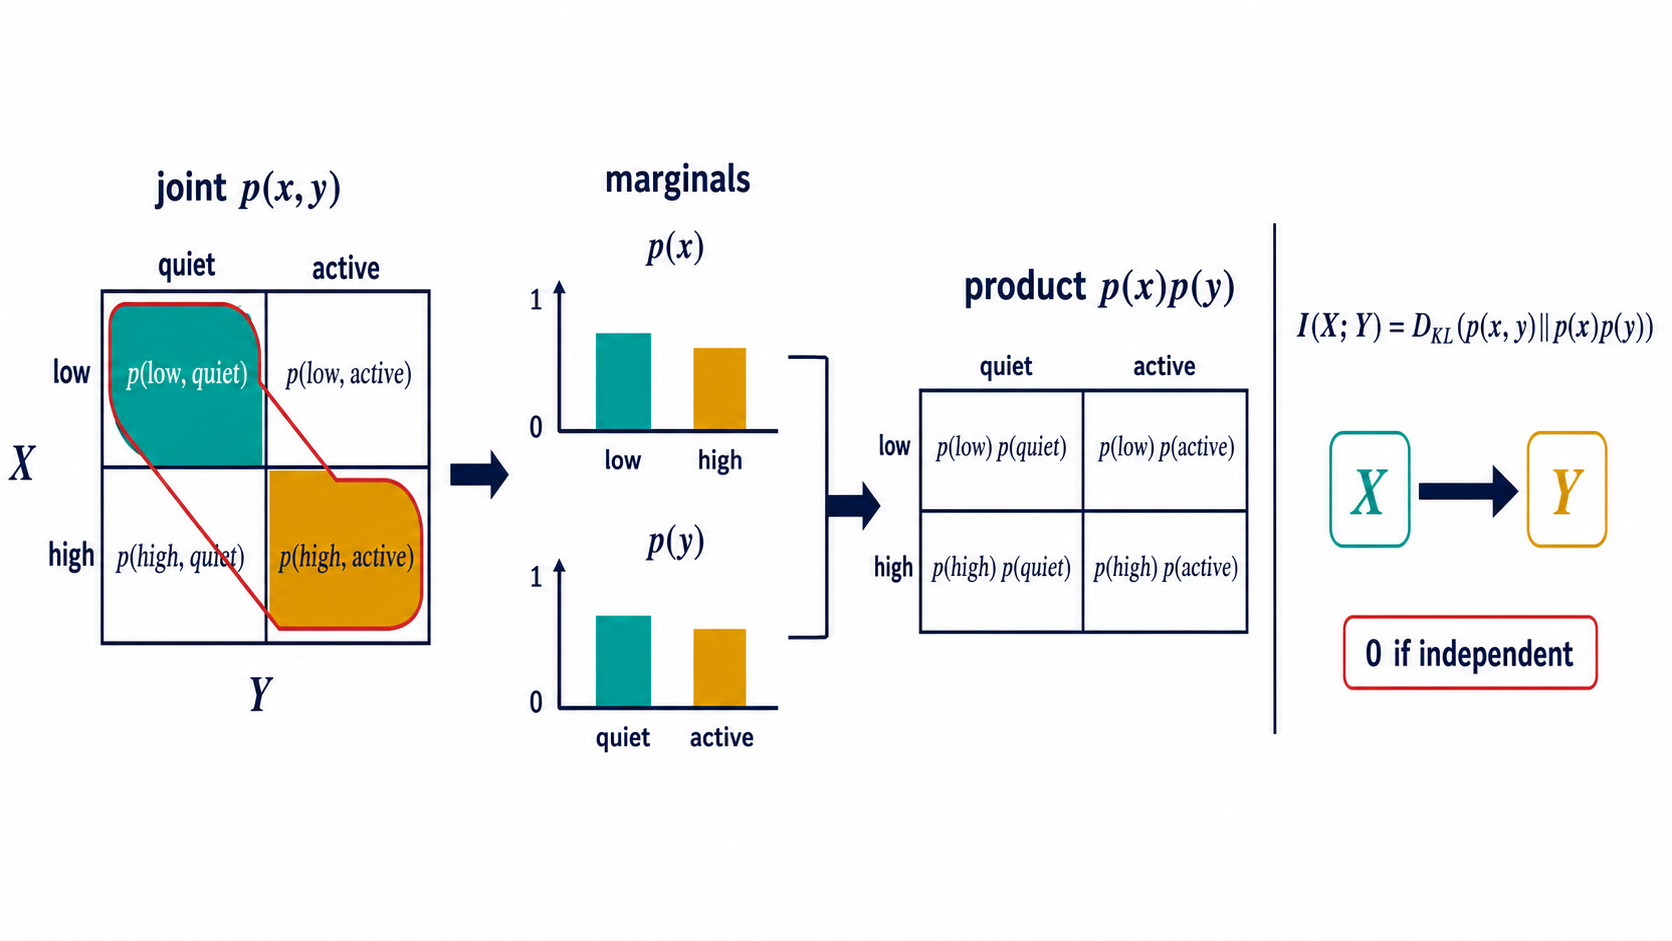
\includegraphics[width=0.98\linewidth]{imagegen-figures/ch18-mutual-information-channel.png}
\caption{Mutual information compares the observed joint distribution \(p(x,y)\) with the product distribution \(p(x)p(y)\) that would hold under independence. Diagonal mass in the joint table means the response is informative about the stimulus.}
\label{fig:ch18-mutual-information-channel}
\end{figure}

\paragraph{Formal setup.}
Let \(X\) and \(Y\) be discrete random variables with joint distribution \(p(x,y)\), marginals
\[
p(x)=\sum_y p(x,y),\qquad p(y)=\sum_x p(x,y),
\]
and conditional distribution
\[
p(x\mid y)=\frac{p(x,y)}{p(y)}
\quad\text{when }p(y)>0.
\]
The conditional entropy of \(X\) given \(Y\) is
\[
\boxed{
H(X\mid Y)
=-\sum_{x,y}p(x,y)\log_2 p(x\mid y).
}
\]
The mutual information between \(X\) and \(Y\) is
\[
\boxed{
I(X;Y)
=\sum_{x,y}p(x,y)\log_2\frac{p(x,y)}{p(x)p(y)}.
}
\]
Equivalently,
\[
\boxed{
I(X;Y)
=D_{\mathrm{KL}}(p(x,y)\|p(x)p(y)).
}
\]
Thus mutual information is the KL divergence between the true joint distribution and the joint distribution that would be obtained if \(X\) and \(Y\) were independent.

\paragraph{Core intuition.}
Figure~\ref{fig:ch18-mutual-information-channel} shows the key comparison. The left table is the actual joint distribution. The product table is what the joint distribution would look like if the marginals stayed the same but dependence were removed. Mutual information measures how different those two tables are.

The conditional-entropy view says the same thing in prediction language:
\[
I(X;Y)=H(X)-H(X\mid Y).
\]
If observing \(Y\) leaves uncertainty about \(X\) unchanged, then \(H(X\mid Y)=H(X)\) and mutual information is zero. If observing \(Y\) removes all uncertainty about \(X\), then \(H(X\mid Y)=0\) and mutual information is \(H(X)\).

A common misconception is that mutual information is just correlation. Correlation detects linear association between numerical variables. Mutual information detects any departure from independence, including nonlinear and nonmonotone relationships. Another misconception is that estimating mutual information from finite data is easy. In high dimensions, reliable estimation is difficult and depends strongly on modeling assumptions, binning, or variational bounds.

This section combines Chapter 15's conditioning with Section 18.2's KL divergence. It prepares information bottlenecks, contrastive representation learning, neural coding, and data-processing arguments.

\paragraph{Main derivation: mutual information as entropy reduction.}
Start from the KL form:
\[
I(X;Y)
=\sum_{x,y}p(x,y)\log_2\frac{p(x,y)}{p(x)p(y)}.
\]
Since \(p(x,y)=p(x\mid y)p(y)\),
\[
\frac{p(x,y)}{p(x)p(y)}
=\frac{p(x\mid y)}{p(x)}.
\]
Therefore
\[
I(X;Y)
=\sum_{x,y}p(x,y)\log_2 p(x\mid y)
-\sum_{x,y}p(x,y)\log_2 p(x).
\]
The first term is \(-H(X\mid Y)\). For the second term, summing over \(y\) gives
\[
\sum_y p(x,y)=p(x),
\]
so
\[
-\sum_{x,y}p(x,y)\log_2 p(x)
=-\sum_x p(x)\log_2 p(x)
=H(X).
\]
Thus
\[
\boxed{
I(X;Y)=H(X)-H(X\mid Y).
}
\]
By symmetry, the same argument also gives
\[
I(X;Y)=H(Y)-H(Y\mid X).
\]

\emph{Data-processing consequence.}
If \(X\to Y\to Z\) is a Markov chain, meaning that \(Z\) depends on \(X\) only through \(Y\), then
\[
\boxed{
I(X;Z)\le I(X;Y).
}
\]
A proof sketch uses the chain rule for mutual information:
\[
I(X;Y,Z)=I(X;Z)+I(X;Y\mid Z)
\]
and also
\[
I(X;Y,Z)=I(X;Y)+I(X;Z\mid Y).
\]
The Markov condition gives \(I(X;Z\mid Y)=0\), while conditional mutual information is nonnegative. Hence
\[
I(X;Z)\le I(X;Y).
\]
Processing cannot create new information about \(X\) beyond what was already present in \(Y\), unless the processing step receives additional information.

\paragraph{Worked examples.}
\emph{Small joint-table example.}
Let \(X\in\{\text{low},\text{high}\}\) be a stimulus and \(Y\in\{\text{quiet},\text{active}\}\) be a response. Suppose
\[
\begin{array}{c|cc}
 & \text{quiet} & \text{active}\\
\hline
\text{low} & 0.4 & 0.1\\
\text{high} & 0.1 & 0.4
\end{array}
\]
Both marginals are uniform: \(p(x)=1/2\) and \(p(y)=1/2\). If \(X\) and \(Y\) were independent, every cell would have probability \(1/4\). The mutual information is
\[
I(X;Y)
=2(0.4)\log_2\frac{0.4}{0.25}
+2(0.1)\log_2\frac{0.1}{0.25}
\approx 0.278\ \text{bits}.
\]
The response is informative but not perfectly informative.

\emph{Conditional-entropy check.}
For the same table, \(H(X)=1\) bit because the stimulus is uniform. Given \(Y=\text{quiet}\), the conditional distribution of \(X\) is
\[
P(X=\text{low}\mid Y=\text{quiet})=0.8,\qquad
P(X=\text{high}\mid Y=\text{quiet})=0.2.
\]
The same entropy occurs for \(Y=\text{active}\). Thus
\[
H(X\mid Y)
=-0.8\log_2(0.8)-0.2\log_2(0.2)
\approx 0.722\ \text{bits},
\]
and
\[
I(X;Y)=1-0.722\approx 0.278\ \text{bits}.
\]

\emph{Neural coding example.}
In a neural coding experiment, \(X\) may be the stimulus orientation and \(Y\) may be a population response vector after binning or modeling. The joint distribution \(p(x,y)\) is estimated from repeated trials or from an encoding model. Mutual information measures how much the response reduces uncertainty about the stimulus. A neuron with high firing-rate variability may still carry information if different stimuli shift the response distribution in distinguishable ways.

\emph{Representation-learning example.}
Let \(X\) be an input, \(Z=f_\theta(X)\) be a learned representation, and \(Y\) be a label. Representation learning often tries to keep information about \(Y\) while discarding irrelevant details of \(X\). In information-bottleneck language, one balances a predictive term related to \(I(Z;Y)\) against a compression term related to \(I(Z;X)\). The random variable \(Z\) is the hidden representation, not an abstract metaphor.

\paragraph{ML/DL/neuroscience connections.}
In neuroscience, mutual information quantifies neural coding by mapping stimulus variables to \(X\) and responses to \(Y\). In deep learning, it helps express questions about what a layer representation retains about inputs, labels, or nuisance variables. In self-supervised learning, contrastive objectives can be viewed as optimizing bounds related to mutual information, though the bound and estimator matter. In experimental design, one can choose stimuli that are expected to produce responses with high information about the latent quantity of interest.

\paragraph{Exercises.}
\begin{enumerate}[label=\textbf{18.3.\arabic*.}, leftmargin=*]
\item \textbf{Mechanical.} For a joint distribution with \(p(0,0)=p(0,1)=p(1,0)=p(1,1)=1/4\), compute \(I(X;Y)\).
\item \textbf{Proof or derivation.} Starting from \(I(X;Y)=D_{\mathrm{KL}}(p(x,y)\|p(x)p(y))\), derive \(I(X;Y)=H(Y)-H(Y\mid X)\).
\item \textbf{Numerical/computational.} For the table in the worked example, change the diagonal entries to \(0.45\) and the off-diagonal entries to \(0.05\). Compute the new mutual information and compare it with \(0.278\) bits.
\item \textbf{Interpretation.} In a stimulus-response experiment, what does \(I(S;R)=0\) mean about the joint distribution of stimulus \(S\) and response \(R\)?
\item \textbf{Debug the misconception.} A student says, "If \(I(X;Y)\) is large, then \(X\) must cause \(Y\)." Correct the statement using the distinction between dependence and causation.
\end{enumerate}

\subsection{18.4 Fisher geometry and statistical manifolds}

\paragraph{Motivating question.}
When each point is a probability distribution \(p_\theta\), how should we measure small movements, curvature, and gradients on the space of models?

\paragraph{Beginner setup.}
A parameterized statistical model
\[
\{p_\theta:\theta\in\Theta\}
\]
can be viewed as a surface whose points are distributions. This is a \emph{statistical manifold}. The parameter \(\theta\) gives coordinates on the surface, but the coordinates are not the geometry itself. A small parameter step can cause a large distributional change in one region and a small distributional change in another.

The Bernoulli family is the smallest example. The parameter \(\theta\in(0,1)\) gives
\[
p_\theta(1)=\theta,\qquad p_\theta(0)=1-\theta.
\]
Changing \(\theta\) by \(0.05\) near \(\theta=0.5\) is less dramatic than changing it by \(0.05\) near \(\theta=0.01\), because near the boundary one outcome is close to impossible. Fisher information makes this local sensitivity precise.

What to keep in mind: information geometry measures distances between nearby distributions, not merely distances between parameter values. Euclidean distance in parameter space can be misleading when the parameterization stretches or compresses the distribution family.

\begin{figure}[htbp]
\centering
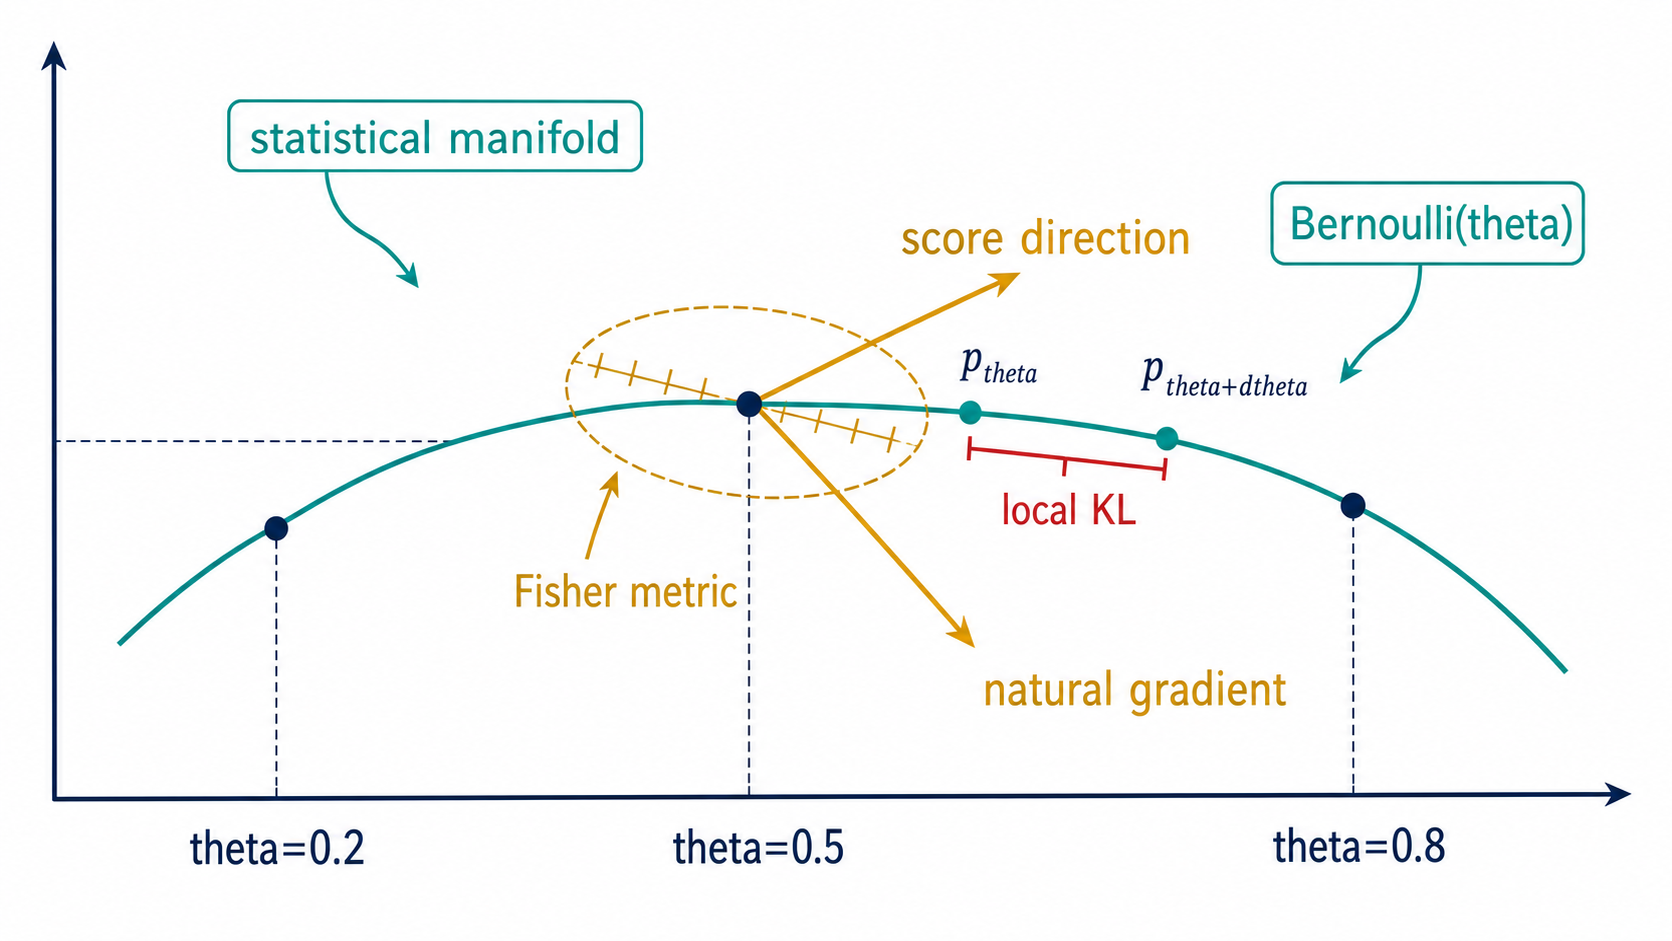
\includegraphics[width=0.98\linewidth]{imagegen-figures/ch18-fisher-statistical-manifold.png}
\caption{A statistical manifold is a parameterized family of probability distributions. Fisher information supplies the local metric: nearby parameter changes are measured by the KL divergence they create between nearby distributions. Natural-gradient methods rescale parameter updates by this metric.}
\label{fig:ch18-fisher-statistical-manifold}
\end{figure}

\paragraph{Formal setup.}
Let \(\theta\in\Theta\subseteq\mathbb R^d\), and let \(p_\theta(x)\) be a differentiable family of probability distributions. In this section, use natural logarithms, because Fisher geometry is usually written in nats. The score vector is
\[
s_\theta(x)=\nabla_\theta \log p_\theta(x).
\]
The Fisher information matrix is
\[
\boxed{
\mathcal I(\theta)
=\mathbb E_{p_\theta}\left[s_\theta(X)s_\theta(X)^\top\right].
}
\]
Under regularity conditions, the same matrix is
\[
\mathcal I(\theta)
=-\mathbb E_{p_\theta}\left[\nabla_\theta^2\log p_\theta(X)\right].
\]

The central local-geometry equation is
\[
\boxed{
D_{\mathrm{KL}}(p_\theta\|p_{\theta+d\theta})
=\frac12\, d\theta^\top \mathcal I(\theta)d\theta
+o(\|d\theta\|^2).
}
\]
Thus \(\mathcal I(\theta)\) acts like a metric tensor: it turns a small coordinate displacement \(d\theta\) into a squared local distributional length.

For an objective \(J(\theta)\), the ordinary gradient \(\nabla_\theta J\) depends on the chosen parameter coordinates. The natural gradient rescales by the Fisher metric:
\[
\boxed{
\widetilde{\nabla}J(\theta)=\mathcal I(\theta)^{-1}\nabla_\theta J(\theta),
}
\]
when \(\mathcal I(\theta)\) is invertible. If the Fisher matrix is singular or ill-conditioned, regularization or a pseudoinverse is needed.

\paragraph{Core intuition.}
Figure~\ref{fig:ch18-fisher-statistical-manifold} connects Chapter 10's manifold idea to probability. A coordinate chart labels distributions by \(\theta\). The tangent direction describes an infinitesimal model change. The Fisher metric says how large that tangent vector is when size is measured by local KL divergence.

A common misconception is that Fisher geometry is a new kind of global distance between any two distributions. The equation above is local: it describes nearby distributions up to second order. Another misconception is that natural gradient is simply "a better optimizer." Its actual role is specific: it chooses an update direction that accounts for how parameter changes alter the model distribution.

This section reuses Chapter 17's Fisher information but changes the viewpoint. Chapter 17 used Fisher information to quantify estimator uncertainty. Here the same object becomes a Riemannian metric on a family of distributions.

\paragraph{Main derivation: local KL curvature.}
Let \(d\theta\) be small. Taylor expand the log density around \(\theta\):
\[
\log p_{\theta+d\theta}(x)
=\log p_\theta(x)
+d\theta^\top \nabla_\theta\log p_\theta(x)
+\frac12 d\theta^\top \nabla_\theta^2\log p_\theta(x)d\theta
+o(\|d\theta\|^2).
\]
Now insert this into the KL divergence
\[
D_{\mathrm{KL}}(p_\theta\|p_{\theta+d\theta})
=\mathbb E_{p_\theta}\left[
\log p_\theta(X)-\log p_{\theta+d\theta}(X)
\right].
\]
The zeroth-order terms cancel. The first-order term is
\[
-d\theta^\top\mathbb E_{p_\theta}[\nabla_\theta\log p_\theta(X)].
\]
Under the usual regularity condition, the expected score is zero:
\[
\mathbb E_{p_\theta}[\nabla_\theta\log p_\theta(X)]=0.
\]
The second-order term becomes
\[
-\frac12 d\theta^\top
\mathbb E_{p_\theta}[\nabla_\theta^2\log p_\theta(X)]
d\theta.
\]
Using the Fisher identity
\[
\mathcal I(\theta)
=-\mathbb E_{p_\theta}[\nabla_\theta^2\log p_\theta(X)]
\]
gives
\[
D_{\mathrm{KL}}(p_\theta\|p_{\theta+d\theta})
=\frac12 d\theta^\top\mathcal I(\theta)d\theta
+o(\|d\theta\|^2).
\]
The mechanism is the same as a second-order Taylor approximation from Chapter 10: the local curvature of KL defines the metric.

\paragraph{Worked examples.}
\emph{Small numerical example.}
For a Bernoulli\((\theta)\) model,
\[
\log p_\theta(X)=X\log\theta+(1-X)\log(1-\theta).
\]
The score is
\[
s_\theta(X)=\frac{X}{\theta}-\frac{1-X}{1-\theta}.
\]
Since \(X=1\) with probability \(\theta\) and \(X=0\) with probability \(1-\theta\),
\[
\mathcal I(\theta)
=\theta\left(\frac{1}{\theta}\right)^2
+(1-\theta)\left(\frac{1}{1-\theta}\right)^2
=\frac{1}{\theta(1-\theta)}.
\]
At \(\theta=0.5\), \(\mathcal I(\theta)=4\). At \(\theta=0.1\), \(\mathcal I(\theta)=1/(0.1\cdot 0.9)\approx 11.11\). A small step \(d\theta=0.05\) has approximate local KL
\[
\frac12\mathcal I(\theta)d\theta^2.
\]
This is about \(0.005\) nats at \(\theta=0.5\), but about \(0.0139\) nats at \(\theta=0.1\). The same coordinate step is distributionally larger near the boundary.

\emph{Natural-gradient example.}
Suppose a one-parameter Bernoulli model has objective derivative \(\nabla_\theta J=0.2\). The ordinary gradient step uses \(0.2\) as the local direction. The natural-gradient direction is
\[
\frac{1}{\mathcal I(\theta)}\nabla_\theta J
=\theta(1-\theta)(0.2).
\]
At \(\theta=0.5\), this equals \(0.05\). At \(\theta=0.1\), it equals \(0.018\). The natural gradient takes a smaller coordinate step near the boundary because the Fisher metric says the distribution changes quickly there.

\emph{Neuroscience example.}
Let \(R\) be a neural response and \(s\) a scalar stimulus. A sensory encoding model \(p(r\mid s)\) has Fisher information
\[
\mathcal I(s)
=\mathbb E_{p(r\mid s)}
\left[
\left(\frac{\partial}{\partial s}\log p(r\mid s)\right)^2
\right].
\]
High \(\mathcal I(s)\) means nearby stimuli \(s\) and \(s+ds\) produce response distributions that are locally easy to distinguish. This connects information geometry to neural coding precision and experimental design.

\emph{Deep-learning example.}
For a neural network that outputs a categorical distribution \(p_\theta(y\mid x)\), Fisher information describes how changing weights \(\theta\) changes the predictive distribution, averaged over inputs and labels. Natural-gradient and approximate second-order methods use this geometry to precondition updates, so that a step size corresponds more closely to a change in predictions than to raw Euclidean weight movement.

\paragraph{ML/DL/neuroscience connections.}
In variational inference, local KL curvature describes how changing variational parameters changes the approximate posterior. In deep learning, Fisher-aware optimizers and natural-gradient approximations try to update parameters in a way that respects predictive distribution geometry. In neuroscience, Fisher information is a local measure of how well a neural population can discriminate nearby stimulus values. The mathematical object \(p_\theta\) becomes a likelihood, a predictive network distribution, an approximate posterior, or a response distribution; the Fisher metric measures local distinguishability in each case.

\paragraph{Exercises.}
\begin{enumerate}[label=\textbf{18.4.\arabic*.}, leftmargin=*]
\item \textbf{Mechanical.} Compute \(\mathcal I(\theta)=1/[\theta(1-\theta)]\) for Bernoulli parameters \(\theta=0.25,0.5,0.75\).
\item \textbf{Proof or derivation.} Fill in the Taylor-expansion derivation of local KL curvature and identify where the expected score being zero is used.
\item \textbf{Numerical/computational.} For a Bernoulli model at \(\theta=0.2\), approximate
\[
D_{\mathrm{KL}}(p_\theta\|p_{\theta+0.02})
\]
using \(\frac12\mathcal I(\theta)d\theta^2\). Then compare it with the exact Bernoulli KL formula.
\item \textbf{Interpretation.} In a neural population code, what does high Fisher information about stimulus \(s\) imply about the local distinguishability of nearby stimuli?
\item \textbf{Debug the misconception.} A student says, "A parameter step of size \(0.1\) always means the same amount of model change." Correct the statement using the Fisher metric.
\end{enumerate}

\paragraph{Closing bridge.}
Chapter 18 completes the first probability and statistics arc by turning uncertainty into quantitative geometry. Entropy measures average surprise, cross-entropy and KL divergence measure prediction and coding mismatch, mutual information measures dependence, and Fisher information measures local distinguishability inside a model family. Later chapters on causality, learning theory, variational inference, neural coding, representation learning, and experimental design reuse these ideas whenever a model must ask what is uncertain, what is distinguishable, what is worth measuring, and what has been learned.

\clearpage
